Orthogonal frequency-division multiplexing (OFDM) and the multi user variant OFDMA are in nearly all modern wireless communication systems, including 4G, 5G, and Wi-Fi 6. OFDM is a modulation technique that divides the available spectrum into multiple orthogonal subcarriers. This allows for high spectral efficiency and robustness against frequency-selective fading. OFDMA is a multiple access scheme that allows multiple users to share the same frequency band by assigning different subcarriers to different users.

But lets start with Frequency Division Multiplexing (FDM) first, which is used in FM radio. In FDM the available frequency band is divided into multiple non-overlapping subbands, each of which is used by a different user. Between the subbands are guard bands to prevent interference between the users. This is a very inefficient use of the spectrum.

\begin{figure}[H]
	\centering
	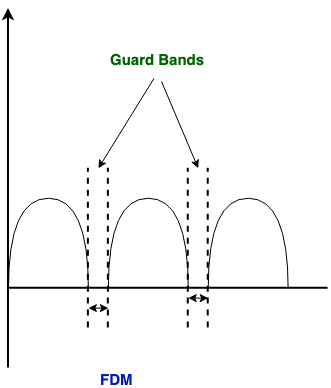
\includegraphics[width=0.4\textwidth]{Figures/fdm.png}
	\caption{Frequency Division Multiplexing}
\end{figure}

OFDM is a more efficient way to divide the spectrum. Instead of using non-overlapping subbands, OFDM divides the spectrum into multiple orthogonal subcarriers. This means that the subcarriers can be spaced closer together, allowing for a higher spectral efficiency. The orthogonality of the subcarriers means that they do not interfere with each other, even when they are spaced closely together. The peaks of the subcarriers line up with the nulls of the other subcarriers, as can be seen in the figure below.

\begin{figure}[H]
	\centering
	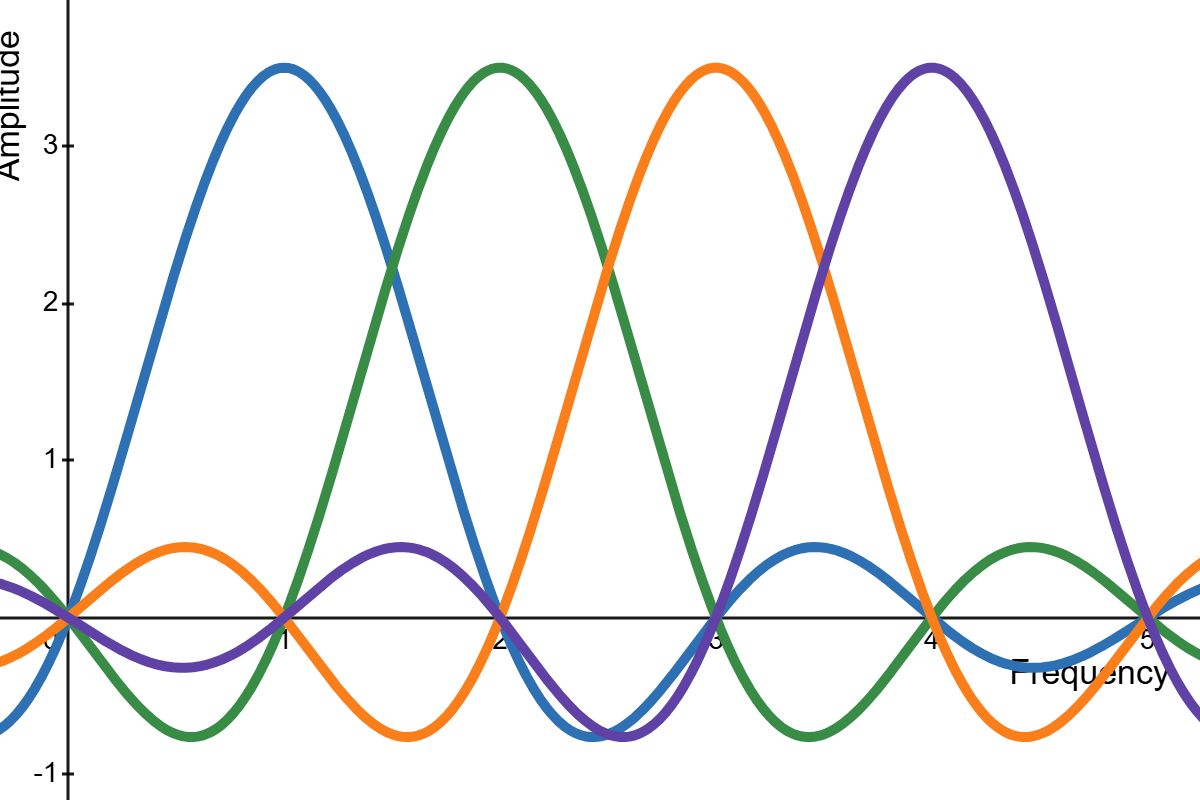
\includegraphics[width=0.4\textwidth]{Figures/ofdm.png}
	\caption{Orthogonal Frequency Division Multiplexing}
\end{figure}